\section{Advanced Topics}
\label{sec:advanced_topics}

Models can be used to describe the dynamic aspects of a system and
transformations can be built in order to simulate the changes in that system
along it's lifetime. Thus, model transformations can be viewed as a kind of
declarative programming where a set of rules define computations as changes in
the information present in the system model \cite{fundamentals_graph_transformations}.

\begin{figure}[h]
\begin{center}
  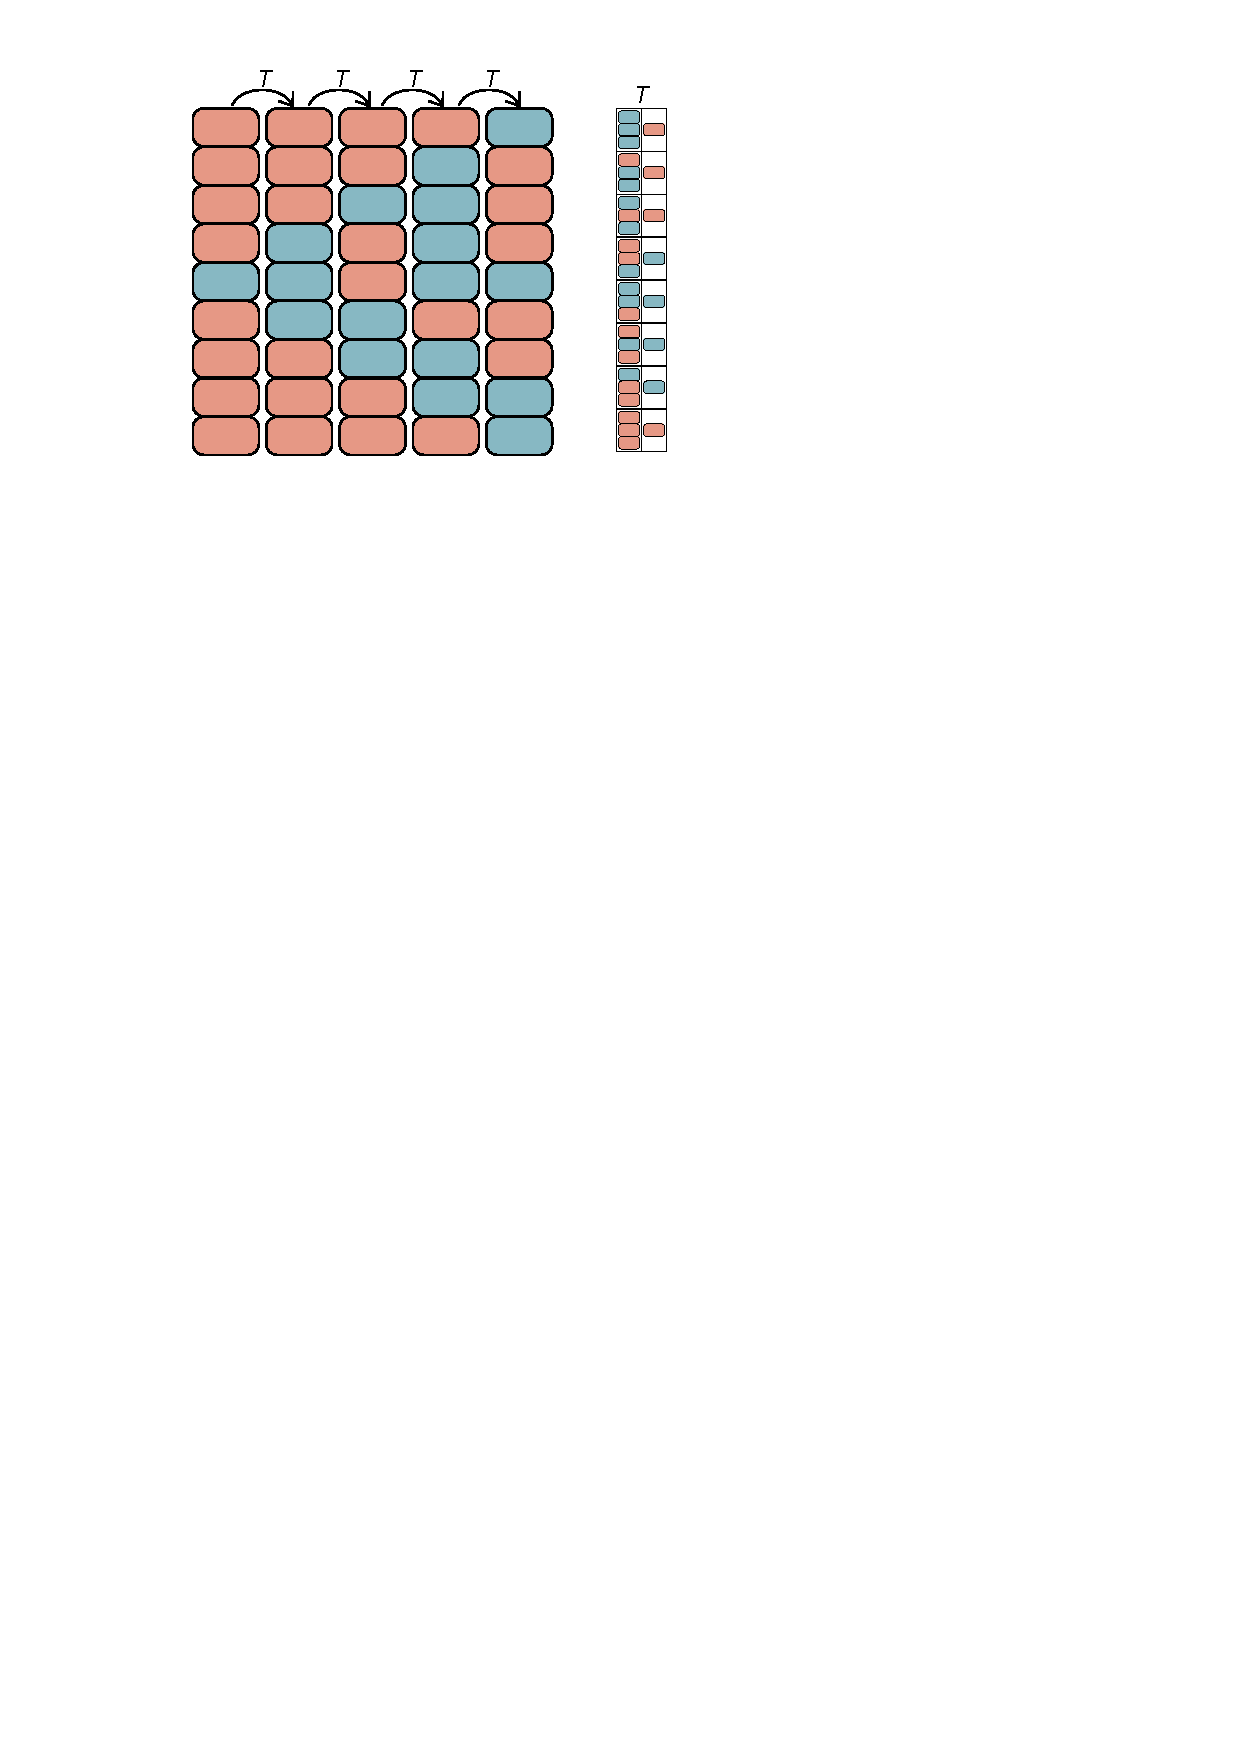
\includegraphics[scale=1, trim=3.0cm 21.7cm 9.5cm 0.9cm,
  clip]{imgs/system_dynamic.pdf}
  \caption{Executing a system by applying the same set of rules $T$ several
  times.}
  \label{fig:system_dynamic}
\end{center}
\end{figure}

In figure \ref{fig:system_dynamic} an example of the changes occurred in a
system by applying the same set of transformations is shown. In this particular
case, the system is represented as the tape of a cellular automaton\footnote{In the context of this
manual, a cellular automaton is a abstract device with an infinite tape
divided in cells that can have two colors. Its behaviour is defined by means of
transformation rules involving a cell and its nearest neighbours.} and it's
behaviour is defined by the set of rules $T$. The next color of a matched cell
is defined according to its own color and its neighbour's. Figure
\ref{fig:system_dynamic} shows the state of the cellular automaton's tape across
four transformations. Curiously, with the set of rules $T$, if you look to
several more transformation applications (with a bigger tape than the one
shown in the figure) you will see that no pattern arrises in the automaton's
behaviour \cite{stephen_wolfram_new_science}.

As you have seen in section \ref{sec:intro}, \emph{DSLTrans} transformations are
no more than models conforming to the \emph{DSLTrans} metamodel. If
\emph{DSLTrans} allows one to create model transformations, then why can't one
build a transformation that handles transformations? In fact, it is perfectly
possible and opens a wide range of possibilities as you will see in this
section.

% TODO Colocar exemplo de automato e maquina de turing e referir a propriedade
% interessante de usar blinks com classes de hierarquia.

\clearpage

\subsection{Finite Deterministic Automata Execution}
\label{subsec:fda_execution}

In this section an example of how a transformation can be used to simulate the behaviour of an abstract mathematical system.

A representation of a Finite Deterministic Automaton (FDA) is shown in figure \ref{fig:automaton_representation} and consists of a reader that crosses a tape in one way, in this case, from left to right, reading a symbol at a time and, depending on the symbols read, it will accept (or not) the sequence present in the tape. 
Figure \ref{fig:automaton_representation_accepted} shows an automaton that has accepted the sequence read from the tape.

\begin{figure}[h]
\begin{center}
  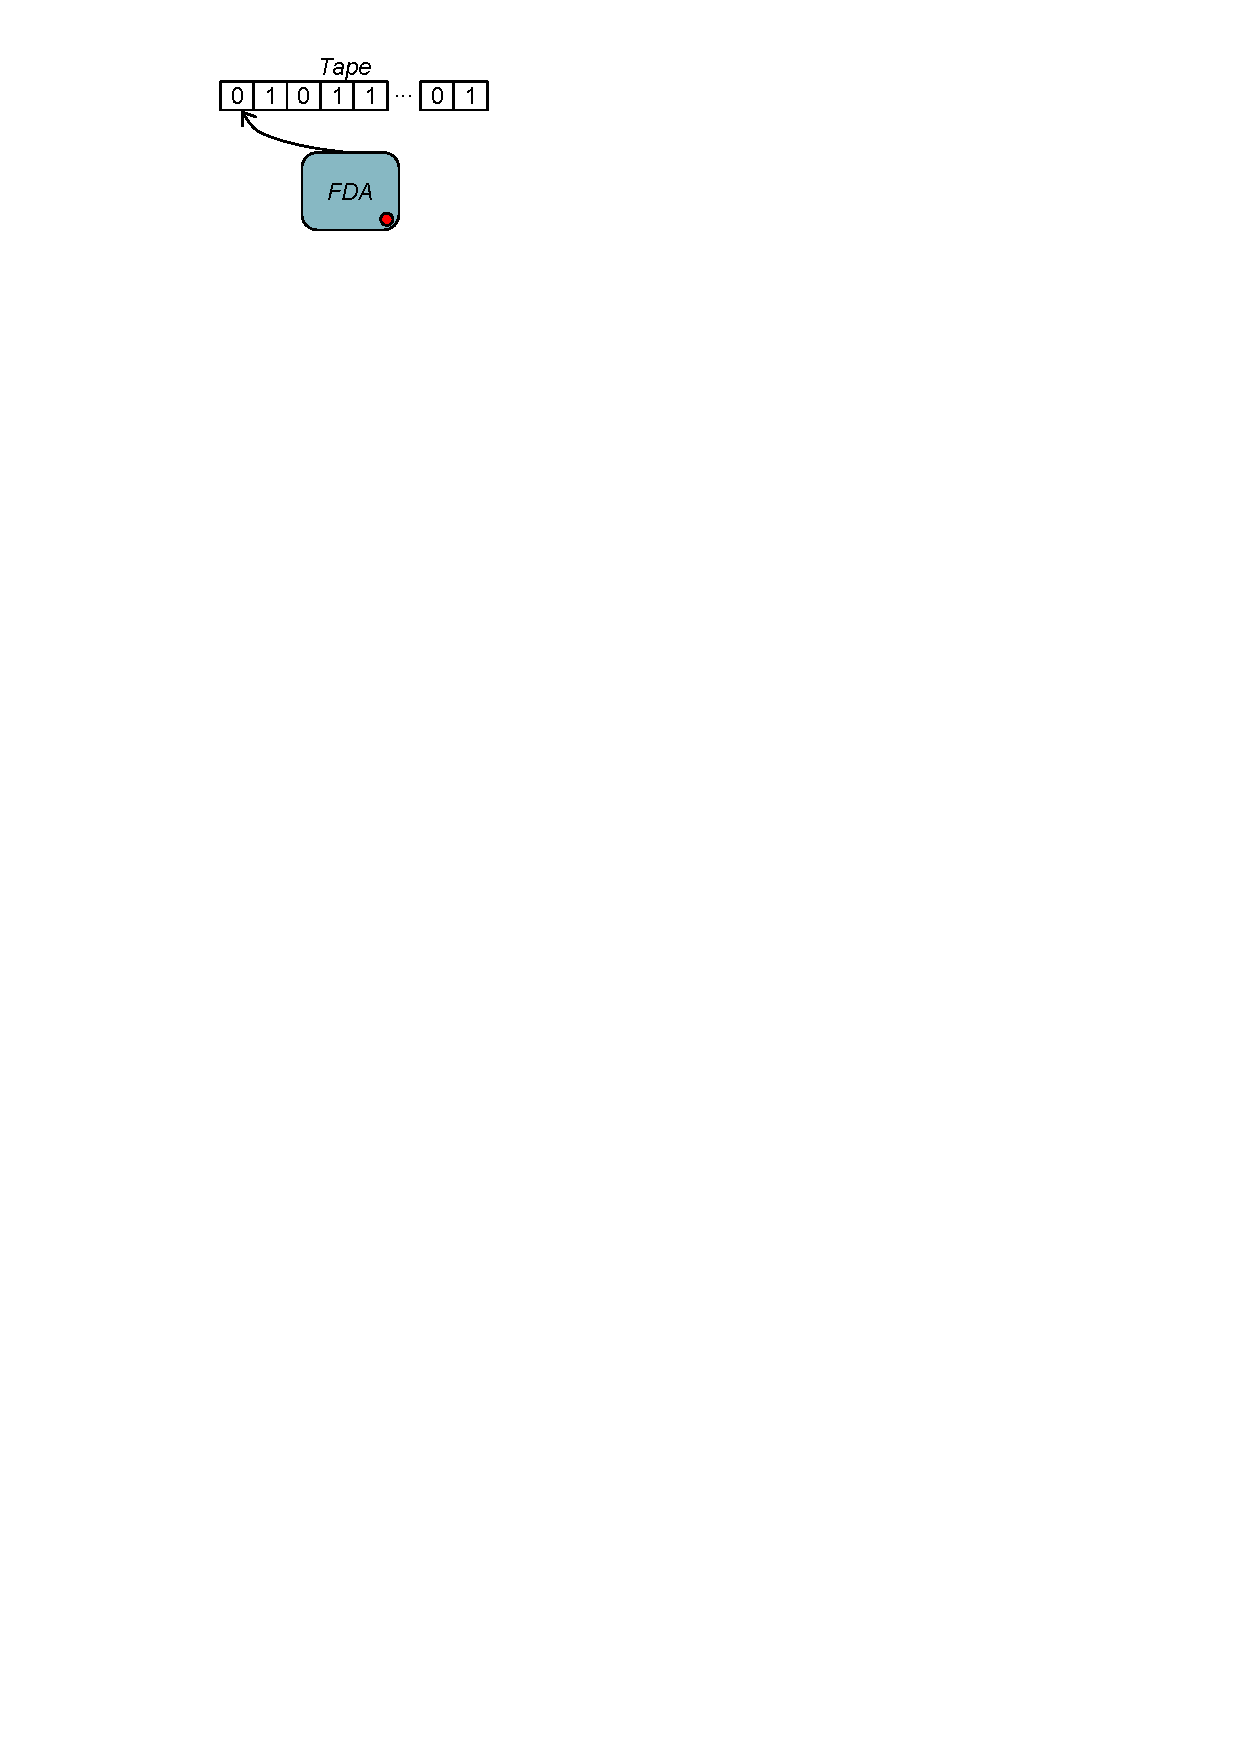
\includegraphics[scale=1, trim=3.5cm 25.4cm 12.4cm 0.6cm,
  clip]{imgs/automaton_representation.pdf}
  \caption{A representation of an automaton system with it's tape and current pointed cell. The red light indicates that the automaton has accepted the sequence read yet.}
  \label{fig:automaton_representation}
\end{center}
\end{figure}

\begin{figure}[h]
\begin{center}
  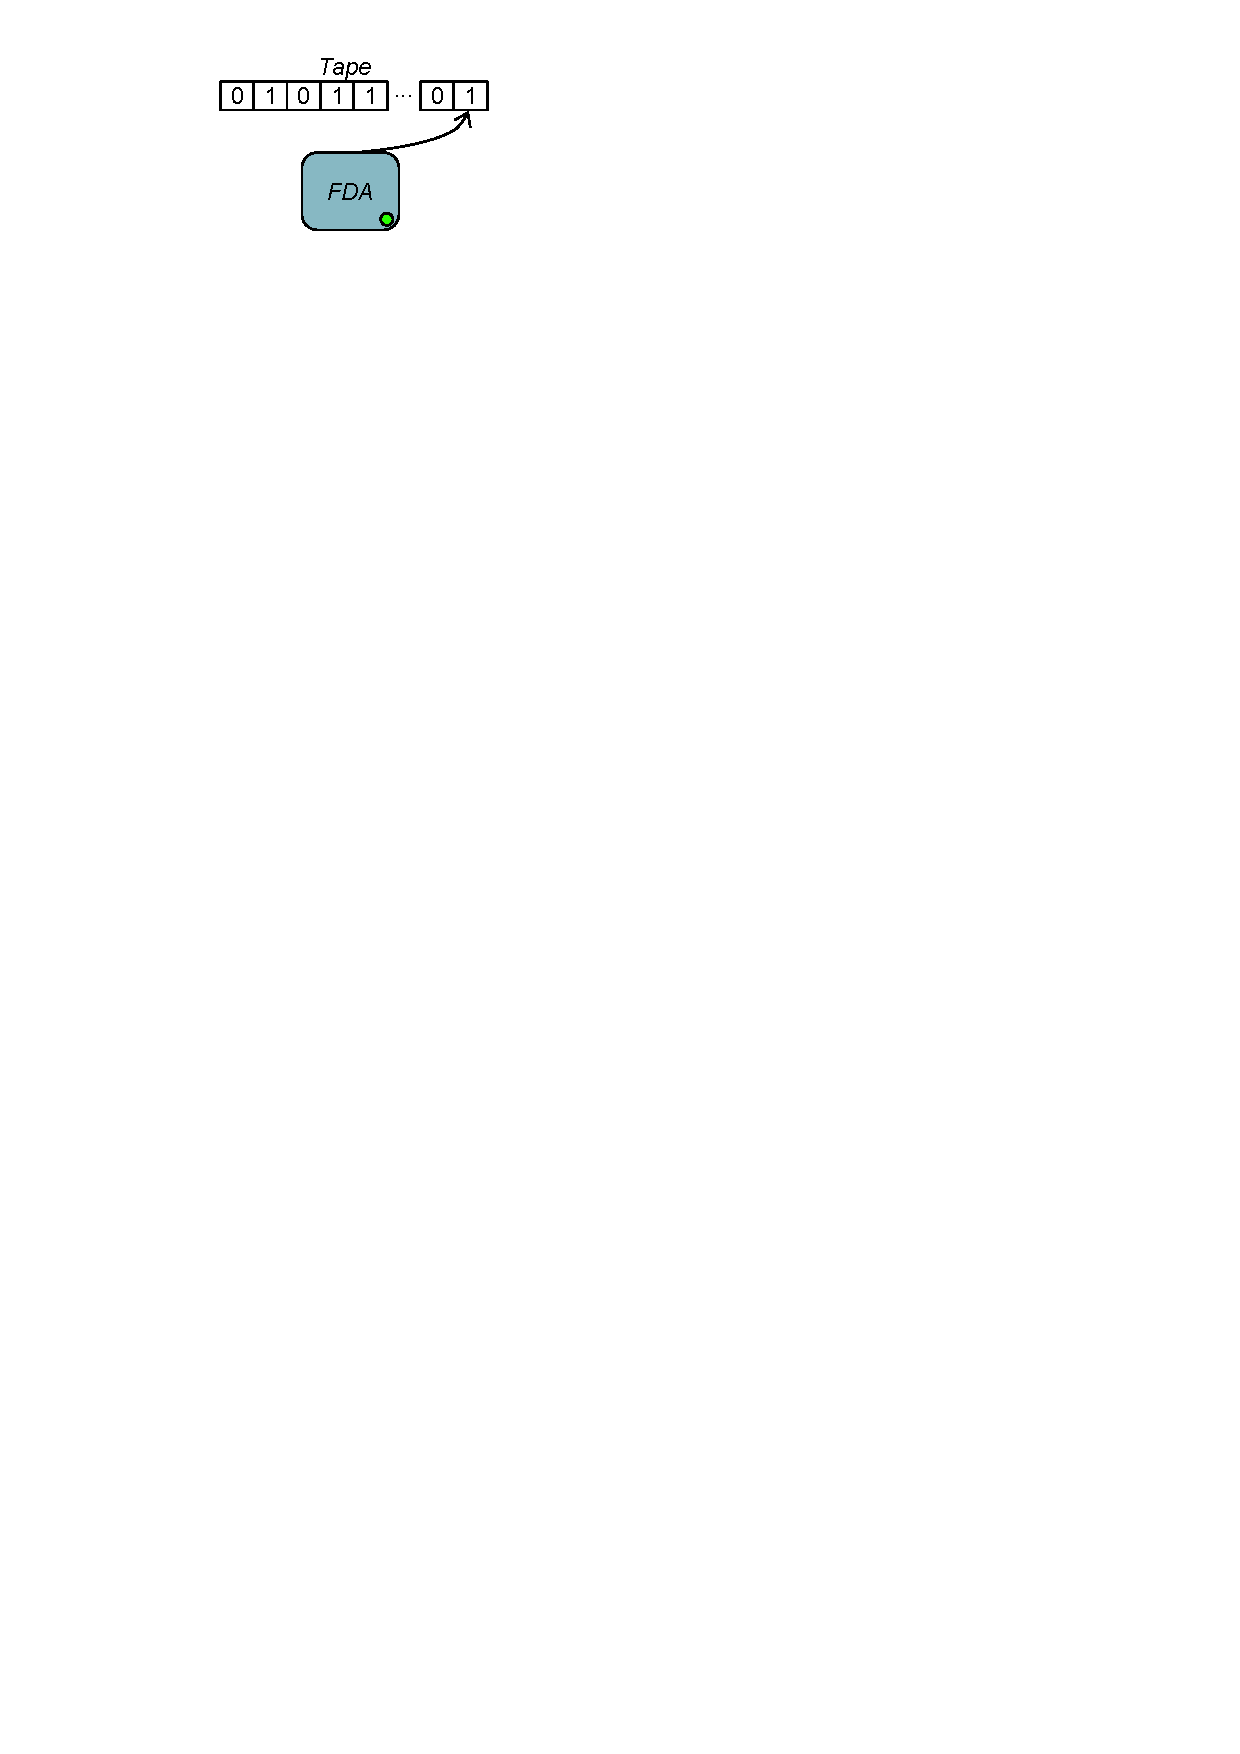
\includegraphics[scale=1, trim=3.5cm 25.4cm 12.4cm 0.6cm,
  clip]{imgs/automaton_representation_accepted.pdf}
  \caption{A representation of a FDA that has accepted the sequence read from the tape.}
  \label{fig:automaton_representation_accepted}
\end{center}
\end{figure}

The acceptance criteria of an automaton can be defined by a labelled graph (hence, a model) with multiple states, an initial state and final/acceptance states. Figure \ref{fig:automaton_behaviour_example} shows a specification of an automaton that accepts only sequences with an even number of $1$'s.


\begin{figure}[h]
\begin{center}
  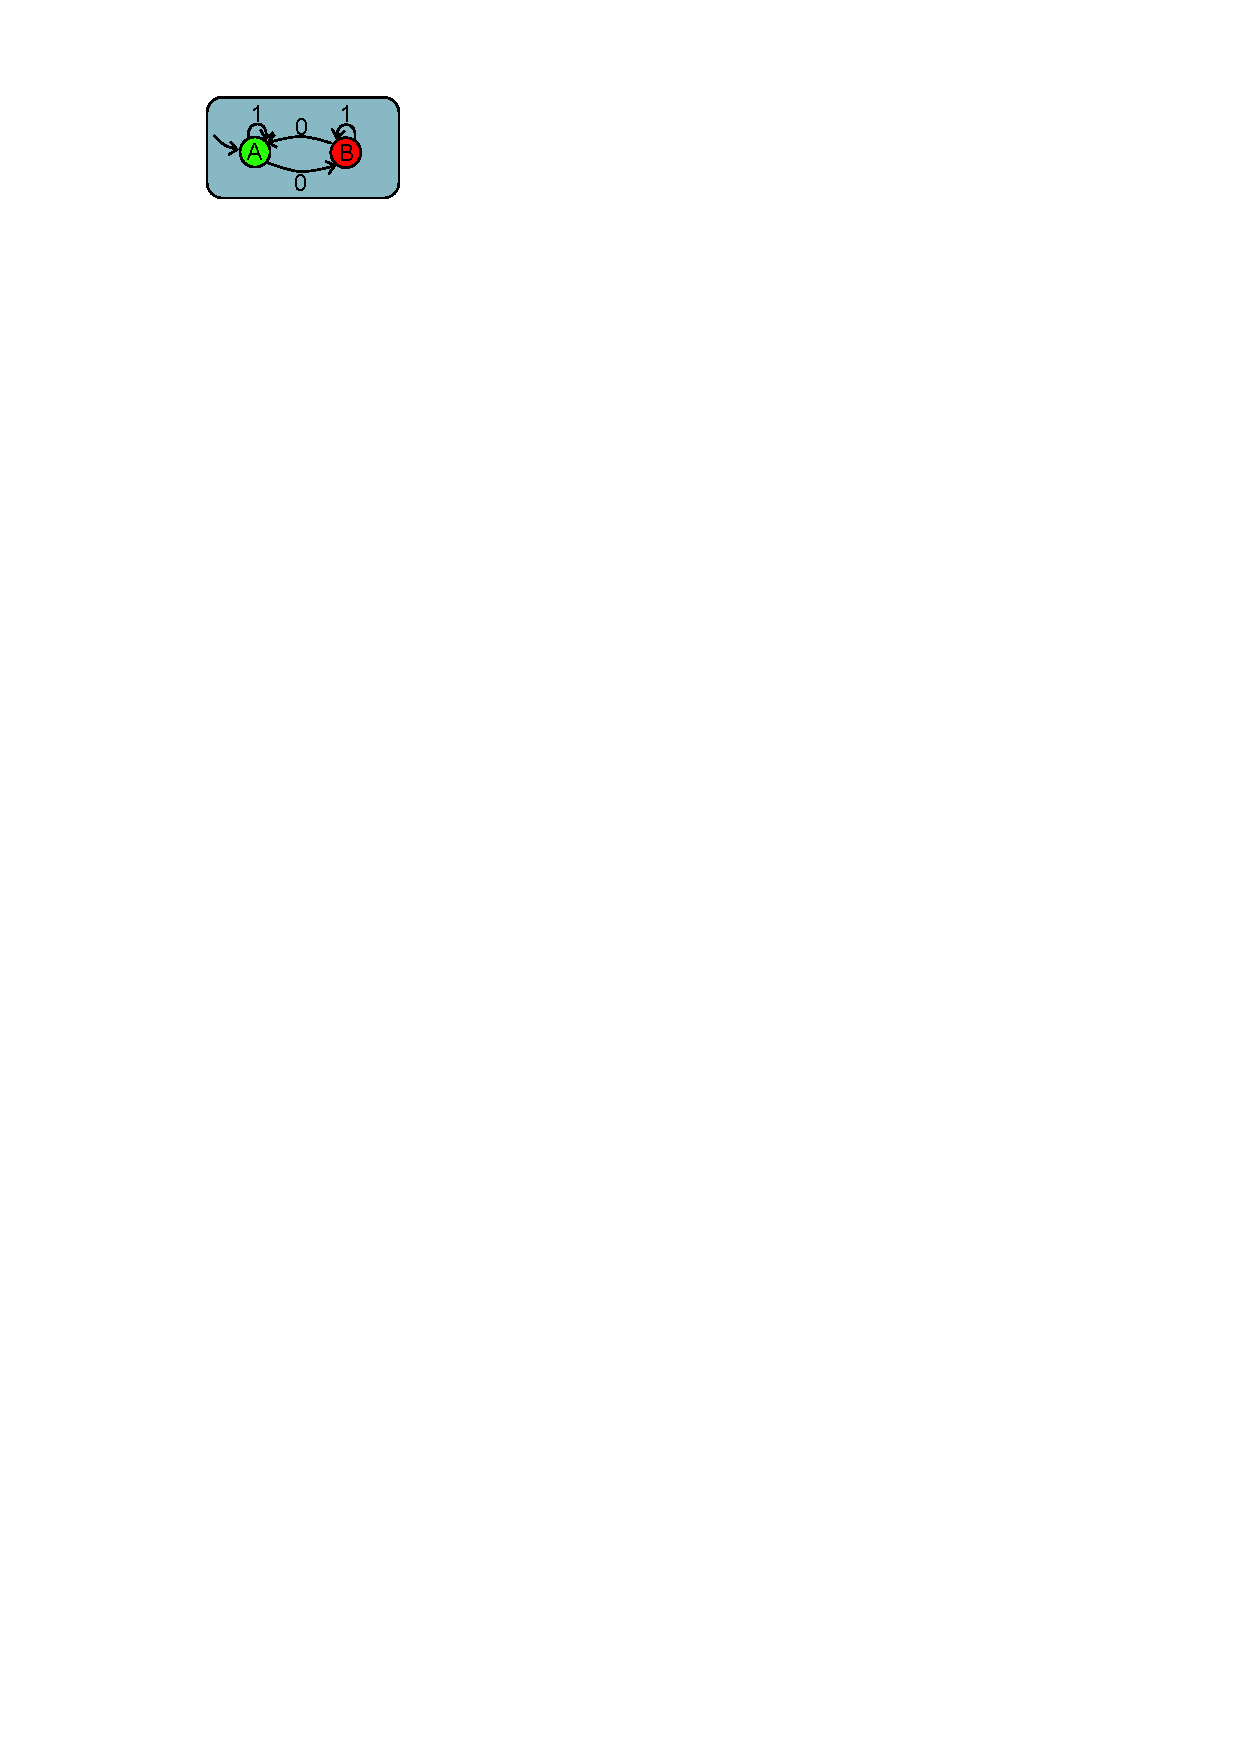
\includegraphics[scale=1, trim=3.2cm 26.1cm 14.1cm 1.3cm,
  clip]{imgs/automaton_behaviour_example.pdf}
  \caption{The behaviour of an automata based on a labelled graph. There are two states, $A$ and $B$, and four transitions, each occurring depending on the current state and the current read symbol ($0$ or $1$).}
  \label{fig:automaton_behaviour_example}
\end{center}
\end{figure}

From a transformation point of view, each step of an automaton execution depends on the current state, the current symbol read from the tape and the transitions available at the current state. The result is a new automaton with the same states and transition from the previous one but with a new current state (that is the target of the executed transition) and a different current symbol. For more information about automata refer to 
\cite{intro_computational_theory}.

In order to show how \emph{DSLTrans} can be used to execute any possible FDA models are needed to represent the state of the automaton across its states. We can either model the tape and the automaton together, or have two separate models: one to represent the tape and the other the automaton. In this example we will opt to follow the second approach. In a latter section (\ref{subsec:turing_machine_trans}) we use a single model.

\begin{figure}[h]
\begin{center}
  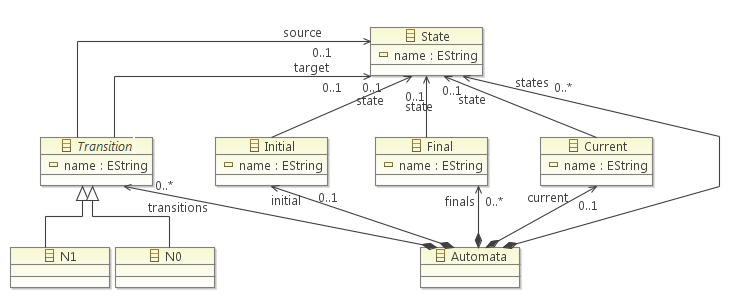
\includegraphics[scale=0.7]{imgs/automata_metamodel.png}
  \caption{Automata Metamodel.}
  \label{fig:automata_metamodel}
\end{center}
\end{figure}

The metamodel for the automaton is shown in figure \ref{fig:automata_metamodel}. It has various states, transitions with labels that are $1$ or $0$. Pointers are needed to represent to the initial, current and final (acceptance) states. These pointer could be attributes of a state but the last are more difficult to change in a transformation but it is perfectly doable.

\begin{figure}[h]
\begin{center}
  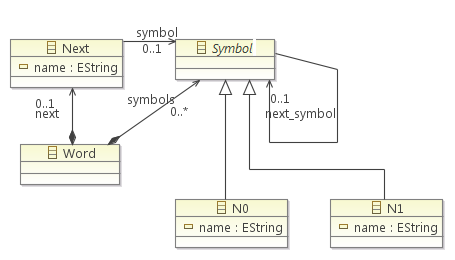
\includegraphics[scale=0.7]{imgs/word_metamodel.png}
  \caption{Word (a.k.a. Tape) Metamodel.}
  \label{fig:word_metamodel}
\end{center}
\end{figure}

Figure \ref{fig:word_metamodel} shows the metamodel used to define a word to be read by the automaton. Notice that to keep a relation of order between the symbols ($0$ or $1$) a \emph{next\_symbol} relation is used. The \emph{Next} pointer indicates the symbol to be read by the automaton in the next step.

In both metamodels, the pointers, states and transitions have names so the models are more readable, they have no influence in the automaton behaviour.

\begin{figure}[h]
\begin{center}
  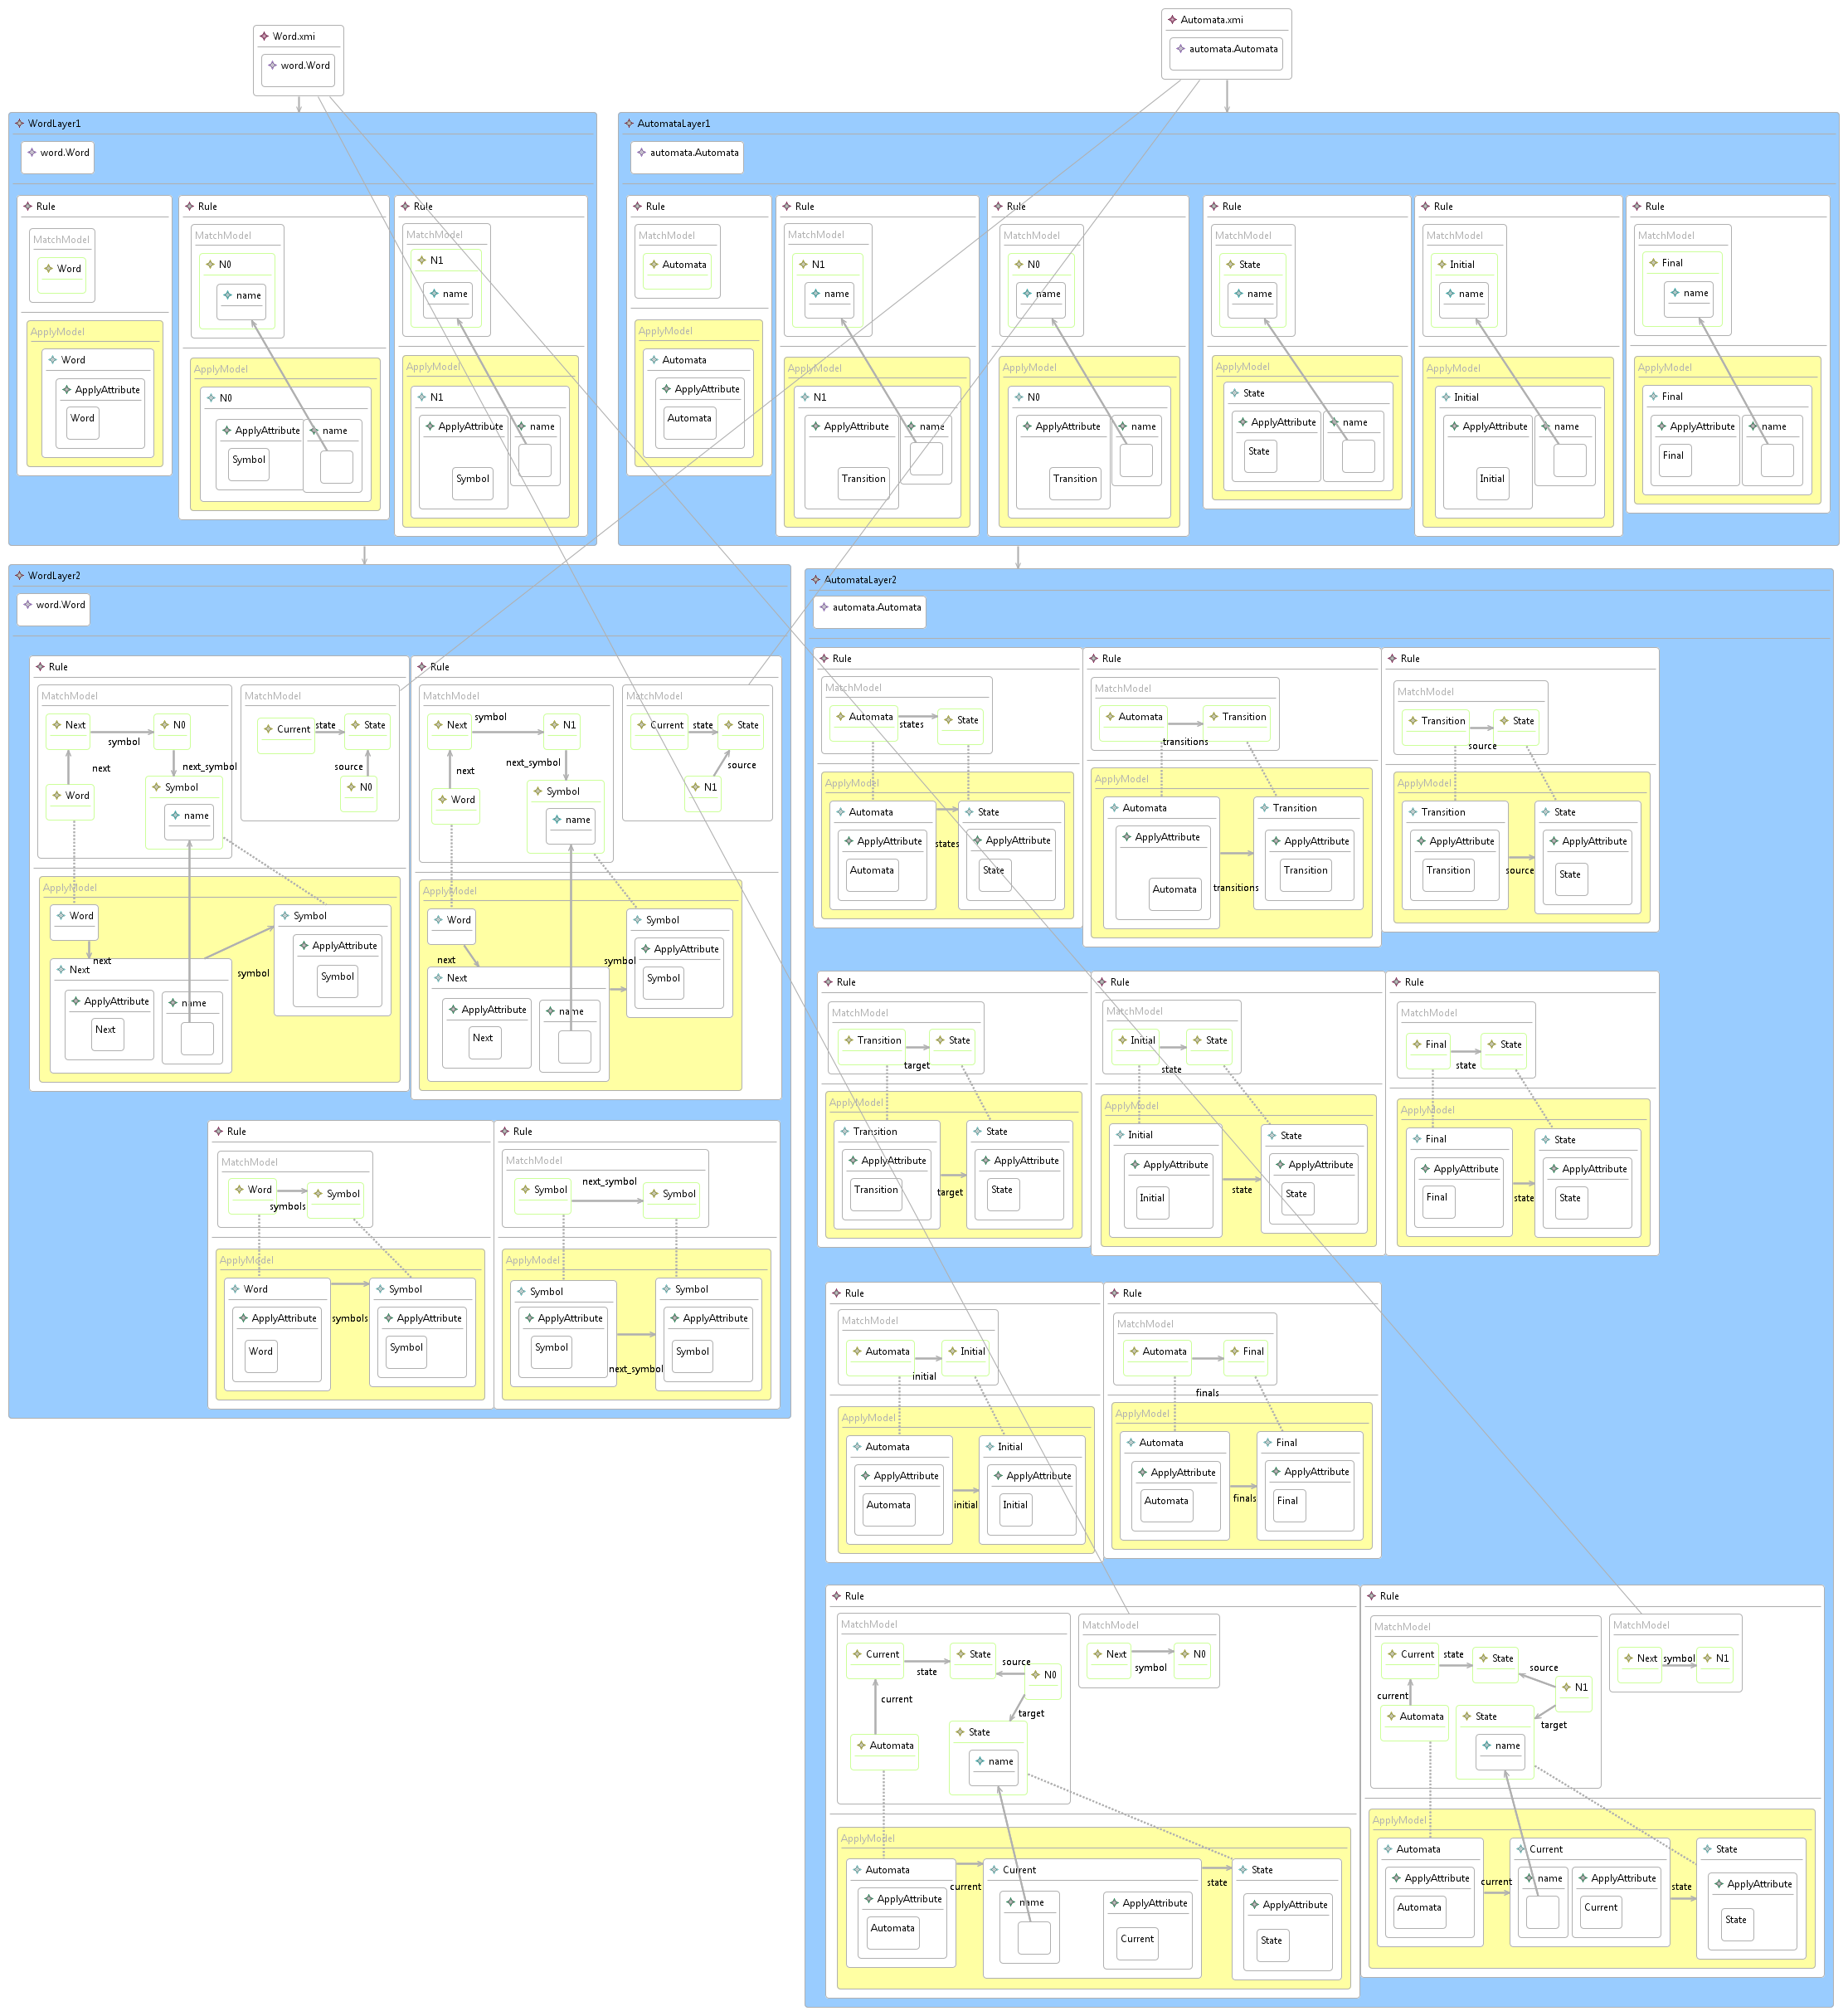
\includegraphics[width=\textwidth]{imgs/ExecuteAutomataTransformationOutline.png}
  \caption{Automata execution transformation outline.}
  \label{fig:ExecuteAutomataTransformationOutline}
\end{center}
\end{figure}

The transformation has two independent flows as can be seen in its outline in figure \ref{fig:ExecuteAutomataTransformationOutline}. That makes sense since there are two models that have to be changed and each flow applies those changes to each model. The tape will have it's \emph{Next} pointer changed according to the automaton and the automaton will have it's \emph{Current} state changed according to the tape, it's current state and the available transitions.

The complete transformation is in the files that come with this manual, please refer to them in the next paragraphs.

Since only the pointers of each model will change and the rest of the elements have to remain intact from the input to the output, the first layer of each flow has the mappings for the elements that remain the same, and copies their attributes.

The second layer of the left flow (the one that changes the word model) has four rules: two of them keep the consistency of the model (order of elements and their connection to the root element) and the other two change the \emph{Next} pointer referring to the current automaton state and the available transitions.

In the right side of the transformation, the second layer has several rules but only two of them actually add any dynamic behaviour to the automaton since the other ones exist only to keep the consistency between input and output models. In those two rules, the \emph{Current} pointer is set according to the current state of the automaton, it's transitions and the symbol read from the word model.

Figures \ref{fig:ExecuteAutomataTransformationOutlineWordRule} and \ref{fig:ExecuteAutomataTransformationOutlineAutomataRule} show the main rules that define the behaviour of this system. All the other rules and layers exist so that the output model remains the same as the input model (except for its pointers).

\begin{figure}[h]
\begin{center}
  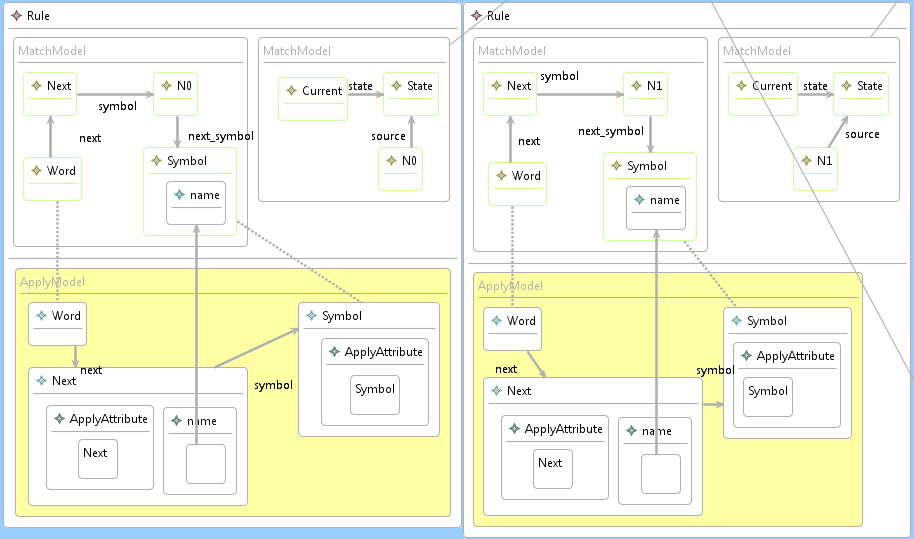
\includegraphics[width=\textwidth]{imgs/ExecuteAutomataTransformationOutlineWordRule.png}
  \caption{The two Word rules the define the \emph{Next} pointer.}
  \label{fig:ExecuteAutomataTransformationOutlineWordRule}
\end{center}
\end{figure}

\begin{figure}[h]
\begin{center}
  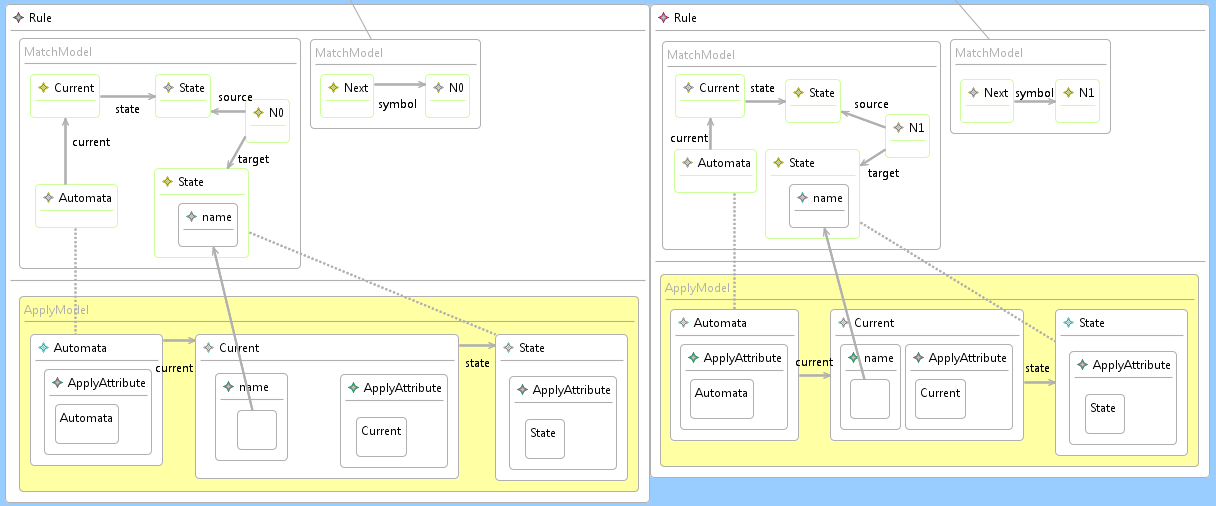
\includegraphics[width=\textwidth]{imgs/ExecuteAutomataTransformationOutlineAutomataRule.png}
  \caption{The two Automata rules the define the \emph{Current} state pointer.}
  \label{fig:ExecuteAutomataTransformationOutlineAutomataRule}
\end{center}
\end{figure}

To see how the models change, figures \ref{fig:initial_automaton_system_state} and \ref{fig:final_automaton_system_state} show the automata and the word models before and after two transformation executions.


\begin{figure}[h]
\begin{center}
  \subfloat[]{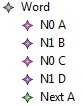
\includegraphics[scale=1]{imgs/automata_model_initial.jpg}}
  \subfloat[]{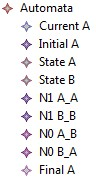
\includegraphics[scale=1]{imgs/word_model_initial.jpg}}
  \caption{Initial system state.}
  \label{fig:initial_automaton_system_state}
\end{center}
\end{figure}


\begin{figure}[h]
\begin{center}
  \subfloat[]{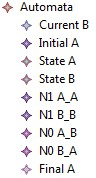
\includegraphics[scale=1]{imgs/automata_model_final.jpg}}
  \subfloat[]{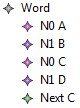
\includegraphics[scale=1]{imgs/word_model_final.jpg}}
  \caption{Final system state.}
  \label{fig:final_automaton_system_state}
\end{center}
\end{figure}

\subsubsection{Conclusions}

Apart from the automaton behaviour simulation using \emph{DSLTrans}, the main ideas to retain from this section are:

\begin{itemize}
\item How to execute two transformations simultaneously using the \emph{PreviousSource} association and different \emph{FilePorts}.
\item How to use the \emph{ExplicitSource} association of a \emph{MatchModel} to control which rules are applied according to an external model. This technique is used in the rules shown in figures \ref{fig:ExecuteAutomataTransformationOutlineAutomataRule} and \ref{fig:ExecuteAutomataTransformationOutlineWordRule}.
\item How to take advantage of class hierarchies in models to reduce the set of rules needed when matching previously generated elements. An example of this technique is shown in figure \ref{fig:ExecuteAutomataTransformationOutlineRuleSymbol} where the left side shows a concrete \emph{Symbol} (\emph{N1}) being generated and the right side shows a rule with a \emph{BackwardLink} matching any \emph{Symbol} generated previously.

\end{itemize}

\begin{figure}[h]
\begin{center}
  \subfloat[Rule in the first layer.]{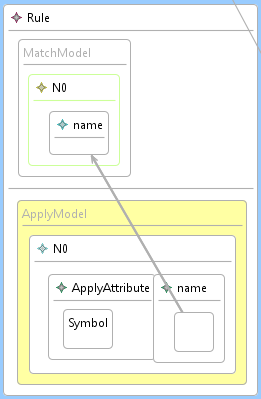
\includegraphics[scale=0.7]{imgs/ExecuteAutomataTransformationOutlineRuleSymbol1.png}}
  \subfloat[Rule in the second layer.]{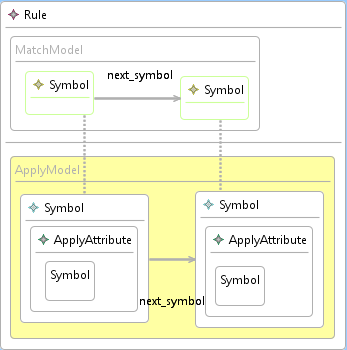
\includegraphics[scale=1]{imgs/ExecuteAutomataTransformationOutlineRuleSymbol2.png}}
  \caption{Using class hierarchy and \emph{BackwardLinks} to reduce the set of rules needed.}
  \label{fig:ExecuteAutomataTransformationOutlineRuleSymbol}
\end{center}
\end{figure}




\clearpage
\subsection{Turing Machine Step Transformation}
\label{subsec:turing_machine_trans}

% Seccao deve ser introduzida explicando que o facto de uma transformacao
% dsltrans ser metamodelada tem vantagens tais como a criacao de higher order
% transformations\ldots



\clearpage
\subsection{High Order Transformations}

% Seccao da um exemplo de construccao de uma higher order transformation (muito
% muito simples)


\clearpage
\subsection{Prototyping Transformations}

\clearpage
\subsubsection{Identity Generation}

\clearpage
\subsubsection{Fixed Identity Generation}

